% Source: graduate-coursework/Sp26/CSCE763/Course_Assignments/HW2/HW2_CSCE_763_solutions.tex

\documentclass[border=4pt]{standalone}
\usepackage{amsmath}
\usepackage{amssymb}
\usepackage{graphicx}
\usepackage{tikz}
\usepackage{xcolor}
\usetikzlibrary{shapes.geometric, arrows.meta, positioning, patterns, calc}

\definecolor{USC_Garnet}{HTML}{73000A}
\definecolor{USC_Sandstorm}{HTML}{FFF2E3}
\definecolor{USC_Black90}{HTML}{363636}
\definecolor{USC_Black70}{HTML}{5C5C5C}
\definecolor{USC_Black50}{HTML}{A2A2A2}
\definecolor{USC_Black10}{HTML}{ECECEC}
\definecolor{USC_Honeycomb}{HTML}{65780B}
\definecolor{USC_Atlantic}{HTML}{466A9F}
\definecolor{USC_Congaree}{HTML}{1F414D}
\definecolor{USC_Rose}{HTML}{CC2E40}
\definecolor{USC_Grass}{HTML}{CED318}
\definecolor{USC_Horseshoe}{HTML}{65780B}
\definecolor{outputbg}{RGB}{245,245,245}

\begin{document}
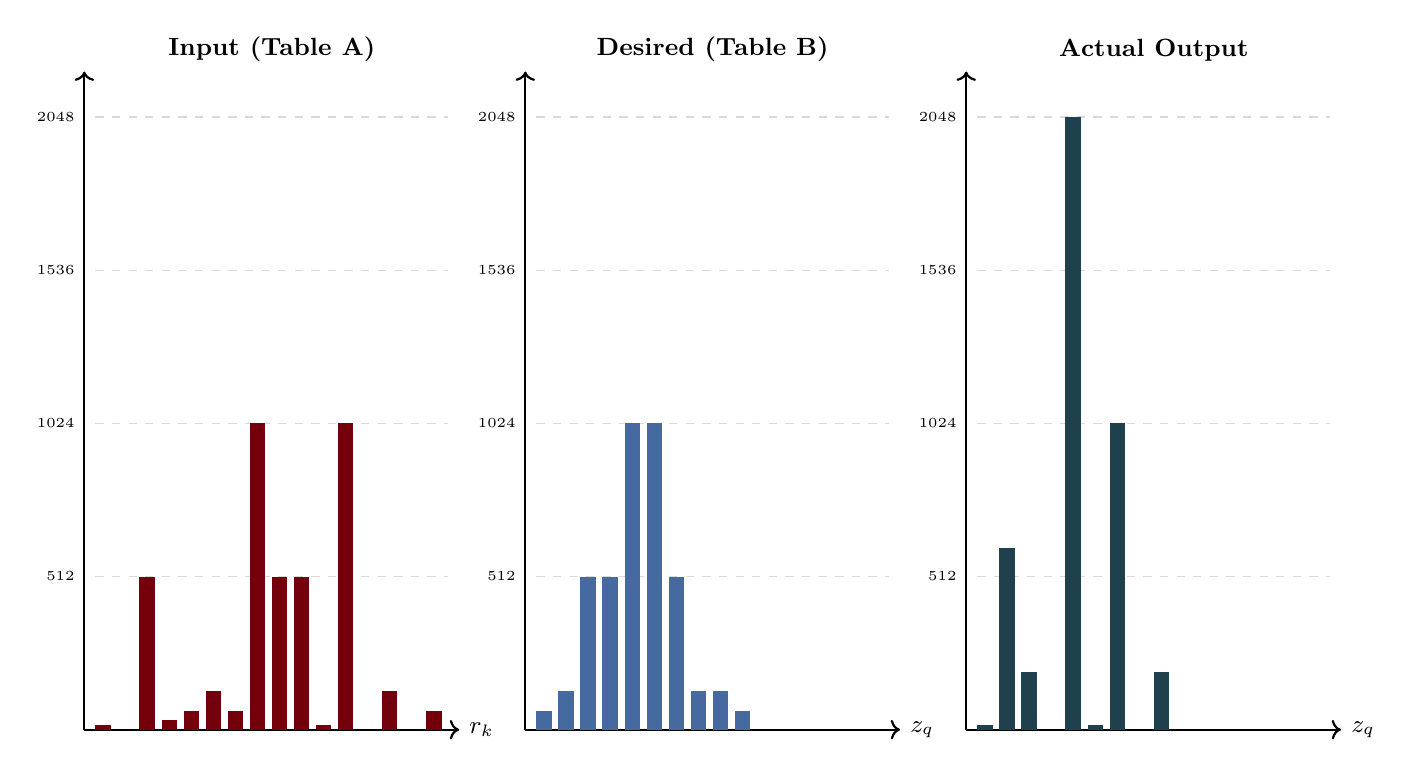
\begin{tikzpicture}[x=0.28cm, y=0.0038cm]
% Helper: draw a single histogram panel
% --- Panel 1: Input (Table A) ---
\begin{scope}[shift={(0,0)}]
\draw[->, thick] (-0.5,0) -- (16.5,0) node[right, font=\small] {$r_k$};
\draw[->, thick] (-0.5,0) -- (-0.5,2200);
\node[above, font=\small\bfseries] at (8,2200) {Input (Table A)};
\foreach \y in {512,1024,1536,2048} {
  \draw[dashed, gray!30] (0,\y) -- (16,\y);
  \node[left, font=\tiny] at (-0.5,\y) {\y};
}
% Bars: r_k -> n_k
\fill[USC_Garnet] (0,0) rectangle (0.7,16);
% r1=0 skip
\fill[USC_Garnet] (2,0) rectangle (2.7,512);
\fill[USC_Garnet] (3,0) rectangle (3.7,32);
\fill[USC_Garnet] (4,0) rectangle (4.7,64);
\fill[USC_Garnet] (5,0) rectangle (5.7,128);
\fill[USC_Garnet] (6,0) rectangle (6.7,64);
\fill[USC_Garnet] (7,0) rectangle (7.7,1024);
\fill[USC_Garnet] (8,0) rectangle (8.7,512);
\fill[USC_Garnet] (9,0) rectangle (9.7,512);
\fill[USC_Garnet] (10,0) rectangle (10.7,16);
\fill[USC_Garnet] (11,0) rectangle (11.7,1024);
% r12=0 skip
\fill[USC_Garnet] (13,0) rectangle (13.7,128);
% r14=0 skip
\fill[USC_Garnet] (15,0) rectangle (15.7,64);
\end{scope}
% --- Panel 2: Desired (Table B) ---
\begin{scope}[shift={(20,0)}]
\draw[->, thick] (-0.5,0) -- (16.5,0) node[right, font=\small] {$z_q$};
\draw[->, thick] (-0.5,0) -- (-0.5,2200);
\node[above, font=\small\bfseries] at (8,2200) {Desired (Table B)};
\foreach \y in {512,1024,1536,2048} {
  \draw[dashed, gray!30] (0,\y) -- (16,\y);
  \node[left, font=\tiny] at (-0.5,\y) {\y};
}
\fill[USC_Atlantic] (0,0) rectangle (0.7,64);
\fill[USC_Atlantic] (1,0) rectangle (1.7,128);
\fill[USC_Atlantic] (2,0) rectangle (2.7,512);
\fill[USC_Atlantic] (3,0) rectangle (3.7,512);
\fill[USC_Atlantic] (4,0) rectangle (4.7,1024);
\fill[USC_Atlantic] (5,0) rectangle (5.7,1024);
\fill[USC_Atlantic] (6,0) rectangle (6.7,512);
\fill[USC_Atlantic] (7,0) rectangle (7.7,128);
\fill[USC_Atlantic] (8,0) rectangle (8.7,128);
\fill[USC_Atlantic] (9,0) rectangle (9.7,64);
\end{scope}
% --- Panel 3: Actual Output ---
\begin{scope}[shift={(40,0)}]
\draw[->, thick] (-0.5,0) -- (16.5,0) node[right, font=\small] {$z_q$};
\draw[->, thick] (-0.5,0) -- (-0.5,2200);
\node[above, font=\small\bfseries] at (8,2200) {Actual Output};
\foreach \y in {512,1024,1536,2048} {
  \draw[dashed, gray!30] (0,\y) -- (16,\y);
  \node[left, font=\tiny] at (-0.5,\y) {\y};
}
\fill[USC_Congaree] (0,0) rectangle (0.7,16);
\fill[USC_Congaree] (1,0) rectangle (1.7,608);
\fill[USC_Congaree] (2,0) rectangle (2.7,192);
\fill[USC_Congaree] (4,0) rectangle (4.7,2048);
\fill[USC_Congaree] (5,0) rectangle (5.7,16);
\fill[USC_Congaree] (6,0) rectangle (6.7,1024);
\fill[USC_Congaree] (8,0) rectangle (8.7,192);
\end{scope}
\end{tikzpicture}
\end{document}
